\documentclass[10pt,twocolumn,letterpaper]{article}

\usepackage{cvpr}
\usepackage{times}
\usepackage{epsfig}
\usepackage{graphicx}
\usepackage{amsmath}
\usepackage{amssymb}
\usepackage{booktabs}

% Include other packages here, before hyperref.

% If you comment hyperref and then uncomment it, you should delete
% egpaper.aux before re-running latex.  (Or just hit 'q' on the first latex
% run, let it finish, and you should be clear).
\usepackage[breaklinks=true,bookmarks=false]{hyperref}

\cvprfinalcopy % *** Uncomment this line for the final submission

\def\cvprPaperID{****} % *** Enter the CVPR Paper ID here
\def\httilde{\mbox{\tt\raisebox{-.5ex}{\symbol{126}}}}

% Pages are numbered in submission mode, and unnumbered in camera-ready
%\ifcvprfinal\pagestyle{empty}\fi
\setcounter{page}{1}
\begin{document}

%%%%%%%%% TITLE

\title{Modelling and Functional Characterization of the Pyridoxamine Kinase/Phosphomethylpyrimidine Kinase Domain Family}

\author{
Marco Uderzo\\
{\small Department of Mathematics, University of Padua}\\
{\tt\small marco.uderzo@studenti.unipd.it}\\
{\tt\small ID: 2096998} \\
\and
Tanner Graves\\
{\small Department of Mathematics, University of Padua}\\
{\tt\small tanneraaron.graves@studenti.unipd.it}\\
{\tt\small ID: 2073559} \\
\and
Claudio Palmeri \\
{\small Department of Mathematics, University of Padua}\\
{\tt\small claudio.palmeri@studenti.unipd.it}\\
{\tt\small ID: 2062671} \\
}


\maketitle
%\thispagestyle{empty}


%%%%%%%%% ABSTRACT
\begin{abstract}
    This project aims to build a sequence model and provide a comprehensive functional characterization of the Pyridoxamine Kinase/Phosphomethylpyrimidine Kinase domain family. The models' accuracy is benchmarked against Pfam annotations in the SwissProt database. Furthermore, the project delves into the functional and structural properties of the domain family, involving taxonomic lineage analysis, Gene Ontology (GO) annotations assessment, and motif searching. (Include findings in the abstract)
\end{abstract}

%%%%%%%%% BODY TEXT
\section{Introduction}

\subsection{Protein Domains}

In molecular biology, a protein domain represents a conserved part of a protein's sequence and three-dimensional structure, capable of evolving, functioning, and existing independently from the rest of the protein chain. These domains, each forming a stable and compact three-dimensional structure, are essential components in proteins, often occurring in various combinations across different proteins. Domains are fundamental in molecular evolution, serving as versatile building blocks that can be rearranged to form proteins with diverse functions. This adaptability and independence make them crucial in understanding protein structure and function.

\subsection{Pyridoxamine Kinase (CHECK FOR ERRORS)}

Pyridoxamine Kinase/Phosphomethylpyrimidine Kinase family is a group of enzymes that play key roles in various biochemical pathways, particularly in the metabolism of vitamins and coenzymes. This family includes two distinct but related enzymes:

\begin{itemize}
\item \textbf{Pyridoxamine Kinase}: This enzyme is involved in the vitamin B6 metabolism pathway. Vitamin B6 exists in different forms, including pyridoxamine, pyridoxal, and pyridoxine. Pyridoxamine kinase specifically catalyzes the phosphorylation of pyridoxamine, converting it into pyridoxamine 5'-phosphate. This is an important step in the salvage pathway of vitamin B6, which is crucial for its recycling and maintenance within the cell.

\item \textbf{Phosphomethylpyrimidine Kinase}: This enzyme is a part of the thiamine (vitamin B1) biosynthetic pathway. It catalyzes the phosphorylation of hydroxymethylpyrimidine (HMP) to hydroxymethylpyrimidine phosphate. This step is essential in the synthesis of thiamine pyrophosphate (TPP), an active form of vitamin B1. TPP is a vital coenzyme in several enzymatic reactions, particularly those involved in carbohydrate metabolism.
\end{itemize}

Both these enzymes, due to their roles in vitamin metabolism, are crucial for maintaining cellular health and function. Disruptions in these pathways can lead to vitamin deficiencies, affecting numerous biological processes.

\subsection{Objective of the Study}

This project aims to build a sequence model and provide a comprehensive functional characterization of the Pyridoxamine Kinase/Phosphomethylpyrimidine Kinase domain family. (Write a small preamble of the goals of this project, even if it is similar to what is written in the abstract).

\section{Methods and Results}

\subsection{Model Building}

Firstly, we queried \textit{UniProt} to retrieve homologous proteins starting from the \texttt{A0A0J9X285} protein, having Pfam domain \texttt{PF08543}. The search returns 150 proteins, considering only SwissProt entries. We then generated a Multiple Sequence Alignment (MSA) starting from the retrieved hits using Clustal Omega.
(Edited MSA with Jalview?)
A Position-Specific Scoring Matrix (PSSM) was obtained by submitting a query to the \texttt{PSI-BLAST} tool, with the SwissProt database as the reference, and an HMM model was built starting from the MSA. (check this)


\subsection{Model Evaluation}

Using \texttt{hmmsearch}, and starting from the \texttt{PSI-BLAST} hits, we generated the predictions, extracting the list of alignments from the HMM search results, in order to understand the sequence alignments that relate to the Pyridoxamine Kinase/Phosphomethylpyrimidine Kinase domain family.
After defining our ground truth by finding all proteins in \textit{SwissProt} with the \texttt{PF08543} domain, we proceeded to evaluating the PSSM model.



\subsubsection{PSSM Protein-Level Performance Evaluation}

The protein-level performances of the PSSM model are shown in the table below:

\begin{center}
    \begin{tabular}{ccc}
        \toprule
        Metric & Value \\
        \midrule
        Precision & 0.894 \\
        Recall & 0.227 \\
        F1-Score & 0.361 \\
        Balanced Accuracy & 0.613 \\
        MCC & 0.45 \\
        \bottomrule
    \end{tabular}
\end{center} 

\begin{center}
    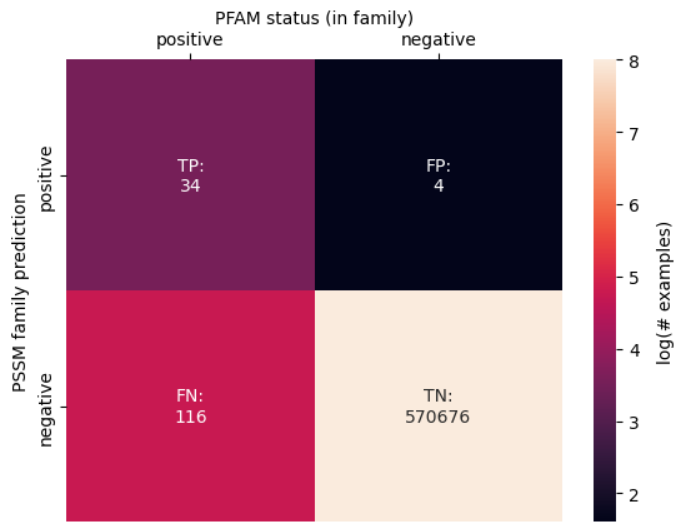
\includegraphics[scale=0.4]{img/pssm_protein_level_eval.png}
\end{center}

The PSSM model has a relatively high number of true negatives (TN: 570,676) and a moderate number of true positives (TP: 34), suggesting that the model is very good at identifying non-members of the family (true negatives) but not as strong at identifying actual members (true positives). The false negatives (FN: 116) are significantly higher than the false positives (FP: 4), indicating that the model tends to miss more actual family members than it incorrectly identifies as family members.

\subsubsection{PSSM Residue-Level Performance Evaluation}

The residue-level performances of the PSSM model are shown in the table below:


\begin{center}
    \begin{tabular}{ccc}
        \toprule
        Metric & Value \\
        \midrule
        Precision & 0.91 \\
        Recall & 0.28
        F1-Score & 0.429 \\
        Balanced Accuracy & 0.64 \\
        MCC & 0.505 \\
        \bottomrule
    \end{tabular}
\end{center} 

\begin{center}
    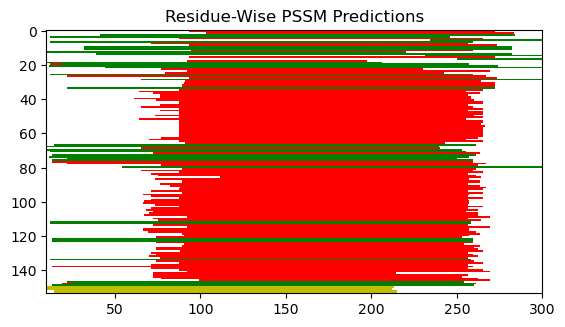
\includegraphics[scale=0.4]{img/pssm_residue_level_eval.png}
\end{center}

To assess the performance of the PSSM model at a detailed, residue-level granularity,
we visualized the overlaps between PFAM domain predictions and actual annotated domains from a database (?). In the plot, each row represents a protein and each column a residue position, color-coded by the prediction accuracy. 

\subsubsection{HMM Performance Evaluation}

\begin{center}
    \begin{tabular}{ccc}
        \toprule
        Metric & Value \\
        \midrule
        Precision & 0.989 \\
        Recall & 0.974
        F1-Score & 0.982 \\
        Balanced Accuracy & 0.987 \\
        MCC & 0.982 \\
        \bottomrule
    \end{tabular}
\end{center} 

\begin{center}
    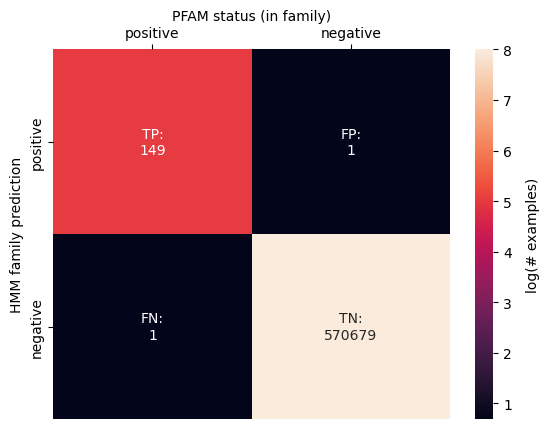
\includegraphics[scale=0.4]{img/hmm_eval.png}
\end{center}

It is worth noting that the HMM model's performance is robust with respect to the starting alignment. (but are our models comparable with the corresponding Pfam?).\\

\subsection{Taxonomy}

\subsection{Functional Enrichment (GO Annotation)}

\subsection{Motifs}



\section{Results}

\section{Discussion}




%-------------------------------------------------------------------------
\section{References}

List and number all bibliographical references in 9-point Times,
single-spaced, at the end of your paper. When referenced in the text,
enclose the citation number in square brackets, for
example.  Where appropriate, include the name(s) of
editors of referenced books.

%{\small
%\bibliographystyle{ieee_fullname}
%\bibliography{egbib}
%}

\end{document}
